%  !TeX  root  =  user_guide.tex

\section{Plugin Oracle Spatial GeoRaster}\label{sec:oracleraster}

% when the revision of a section has been finalized, 
% comment out the following line:
% \updatedisclaimer

Nei database Oracle i dati raster possono essere gestiti come oggetti SDO\_GEORASTER messi 
a disposizione dall'estensione Oracle Spatial. In QGIS il \toolbtntwo{oracle_raster}{Plugin Oracle Spatial GeoRaster} 
è supportato da GDAL e le sue funzionalità dipendono dal database Oracle installato sulla 
propria macchina. 
Il software Oracle è proprietario, sebbene il suo utilizzo sia libero per attività di 
sviluppo e test.

Il comando seguente: 

\begin{verbatim} 
$ gdal_translate -of georaster input_file.tif geor:scott/tiger@orcl
\end{verbatim}

carica un raster nella tabella predefinita GDAL\_IMPORT in una colonna con nome RASTER.

\subsection{Gestire le connessioni}

Assicurarsi che il plugin sia abilitato nel gestore dei plugin (Sezione \ref{sec:load_core_plugin}). 
Prima di caricare un GeoRaster bisogna creare una connessione al database Oracle contente i dati:
L'icona \toolbtntwo{oracle_raster}{Aggiungi layer Oracle GeoRaster} nella barra dei plugin apre la finestra 
di dialogo \dialog}{Scegli Oracle Spatial GeoRaster}. In Connessioni server cliccare su \button{Nuovo} ed 
inserire i parametri di connessione al database (Figura \ref{fig:oracle_create}):

\begin{itemize}[label=--]
\item \textbf{None}: inserire un nome per la connessione.
\item \textbf{Istanza database}: inserire in nome del database cui si intende connettersi.
\item \textbf{Nome utente}: inserire il nome utente.
\item \textbf{Password}: inserire la password.
\end{itemize}

\begin{figure}[ht]
   \centering
   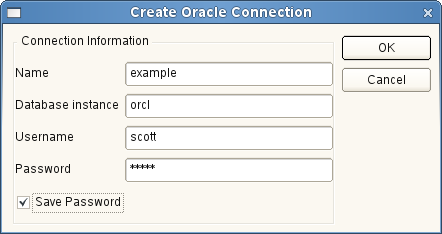
\includegraphics[clip=true, width=9cm]{oracle_create_dialog}   
   \caption{Finestra di dialogo Crea una connessione Oracle \nixcaption}\label{fig:oracle_create}
\end{figure}

Cliccando su \button{OK} i parametri della connessione vengono salvati e si ritorna nella finestra di dialogo 
per la scelta del georaster (Figura \ref{fig:oracle_select}). Selezionare la connessione appena 
impostata e cliccare su \button{Connetti}: per modificare una connessione cliccare su \button{Modifica}, per 
rimuoverla cliccare su \button{Elimina}.

\subsection{Selezionare un GeoRaster}

Stabilita la connessione, il riquadro 'Sottoinsieme di dati' elencherà le tabelle del database contenenti 
colonne georaster compatibili con GDAL.

Selezionare una tabella con il mouse e cliccare su \button{Seleziona}: apparirà un nuovo elenco con i nomi delle 
colonne GeoRaster della tabella selezionata.

Selezionare una colonna con il mouse e cliccare su \button{Seleziona}: apparirà un nuovo elenco contenente 
gli oggetti GeoRaster.

In ogni momento è possibile modificare la selezione per raggiungere direttamente un GeoRaster noto o per 
selezionare un'altra tabella.

\begin{figure}[ht]
   \centering
   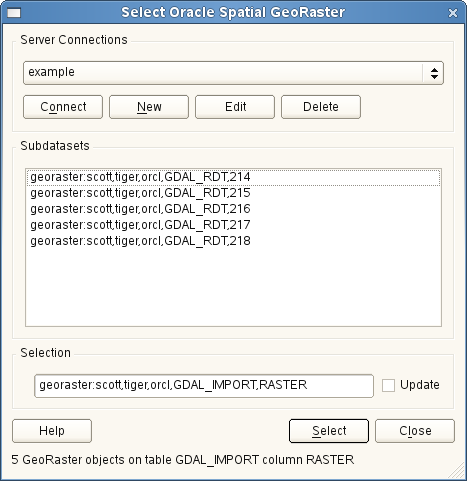
\includegraphics[clip=true, width=9cm]{oracle_select_dialog}   
   \caption{Finestra di dialogo Scegli Oracle Spatial GeoRaster \nixcaption}\label{fig:oracle_select}
\end{figure}

Il testo mostrato nella casella 'Selezione' può essere usato in una clausola SQL WHERE, es:
``geor:scott/tiger@orcl,gdal\_import,raster,geoid=''. Si veda \url{http://www.gdal.org/frmt_georaster.html} 
per ulteriori informazioni.

\subsection{Visualizzare un GeoRaster}

Selezionando un GeoRaster dalla lista appena descritta, esso sarà visualizzato in QGIS. La finestra di dialogo 
per la scelta dei georaster può ora essere chiusa: riaprendola, essa mostrerà la medesima connessione e 
lo stesso elenco di georaster, rendendo semplice la scelta di una nuova immagine dallo stesso contesto.

\textbf{Nota:} I GeoRaster con piramidi vengono visualizzati molto più rapidamente. Le piramidi possono essere 
generate con Oracle PL/SQL oppure con gdaladdo.

Segue un esempio di utilizzo di gdaladdo:

\begin{verbatim}
gdaladdo georaster:scott/tiger@orcl,georaster\_table,georaster,georid=6 -r 
nearest 2 4 6 8 16 32
\end{verbatim}

Questo è, invece, un esempio con PL/SQL: 
\begin{verbatim}
$ sqlplus scott/tiger
SQL> DECLARE
    gr sdo_georaster;
BEGIN
    SELECT image INTO gr FROM cities WHERE id = 1 FOR UPDATE;
    sdo_geor.generatePyramid(gr, 'rLevel=5, resampling=NN');
    UPDATE cities SET image = gr WHERE id = 1;
    COMMIT;
END;
/
\end{verbatim}

\FloatBarrier
